%% Theoretical predictions 
\section{Predictions from Monte Carlo Event Generators}
\subsection{Overview of Monte Carlo Event Generators}
\label{sec:mceg}
Monte Carlo Event Generators (MCEG) play an important role in high energy physics. Generators such as \herwig{}~\cite{Bellm:2017bvx}, \pythia{}~\cite{Sjostrand:2006za} and \SHERPA~\cite{Gleisberg:2008ta} amongst others are essential in data analysis. Together with programs that simulate the detector effects, they are used to estimate the signal and background distributions of various processes. This section gives a brief review of how MCEGs simulate proton-proton collisions, drawing from References~\cite{seymour2013monte,hoche2015introduction,pdg_2021}, to which the readers may refer to for for an in-depth review. 

Protons are composite particles. In order to model how they collide on an event-by-event basis at the LHC, one must model how the partons (valence quarks, sea quarks, and gluons) behave. To achieve this complex goal, the event must be broken up into several phases, each produced via different techniques and occupying a unique region in phase space. QCD is weakly interacting at short distances. Therefore the components of the MCEG dealing with short-distance physics are based on perturbation theory~\cite{pdg}. At larger distances, all soft hadronic phenomena such as hadronization and the formation of the underlying event in hadron collisions cannot be computed from first principles~\cite{pdg}. Instead, one must rely upon other models. This is the general idea behind factorization theorem.

Inside the factorization theorem, an important concept is the Parton Distribution Function (PDF). Written as $f_i(x,\mu_F^2)$, this corresponds to the probability to find a parton of flavour $i$ in the proton as a function of the fraction $x$ of the proton’s momentum carried by the parton and $\mu_F^2$ the energy scale of the hard interaction. $\mu_F^2$ is often referred to as the factorization scale. Since QCD does not predict the parton content of the proton, the shapes of the PDFs are determined by a fit to data from experimental observables in various processes~\cite{placakyte2011parton}.

The event simulation starts at the heart of the collision: the hard scatter. In Figure~\ref{fig:MCEG}, this is the central blob in red. The hard scatter is the one with the largest transfer of energy between the two colliding partons. This is relatively straight-forward to simulate to some fixed order via the matrix element prescription. Nowadays for matrix element calculators, it is standard for most processes to calculate up to Next-to-Leading-Order (NLO), so as to include loop radiative correction. While including higher-order corrections reduces theory uncertainty~\cite{gutschow_lecture}, it is  computationally expensive.

Another important aspect of event generation is the Parton shower, which connects the matrix element to the produced and observed hadrons. These are the squiggly branch structures of Figure~\ref{fig:MCEG}. The parton shower describes what happens to the incoming and outgoing parton of the hard collision~\cite{seymour2013monte}. Since partons are coloured, they behave in a Bremsstrahlung-like fashion and radiate gluons as they move through a collision. Recall from Section~\ref{sec:particlecontent} that gluons can also self interact and emit another gluon, leading to an extended shower of partons that is made up of mostly soft gluons~\cite{seymour2013monte}. The parton shower develops with decreasing values of a parameter that is a
measure of the hardness of interactions~\cite{Nagy:98014034}. It is an evolution in momentum transfer scale that starts from the hard process and works to lower momentum until a point is reached where perturbation theory breaks down~\cite{seymour2013monte}. 

As the parton shower branches, the QCD force grows until confinement takes over and results in the partons grouping together into colour-singlet hadrons, illustrated in bright green in Figure~\ref{fig:MCEG}. This process is described using hadronization models. The hadrons simulated may not be stable, meaning that they decay inside the detector volume. The decays are modelled inside the simulations using information about hadron lifetime, branching ratios and hadron decay width~\cite{Cabras:2743914}. Of course, aside from the hard collision there are lots of secondary interactions between the proton remnants~\cite{seymoure2013monte}. This is referred to as the underlying event, sketched in purple in Figure~\ref{fig:MCEG}. It produces soft hadrons everywhere in the event, which overlie and contaminate the hard process that was already simulated~\cite{seymour2013monte}.

The MCEGs used to simulate four-lepton events for this analysis, along with key parameters such as PDF set and NLO corrections, are summarized in the next section. The MC samples are used in the design and optimization of the analysis, in evaluating the uncertainties, and in correcting the data from detector inefficiency and resolution effects.
\info[inline]{Simulating the hard process is relatively straightforward because Parton Distribution Functions (PDFs) describe partons coming into the process and lowest order perturbation theory gives a probabilistic distribution of the outgoing partons.}

\begin{figure}[htb!]
    \centering
    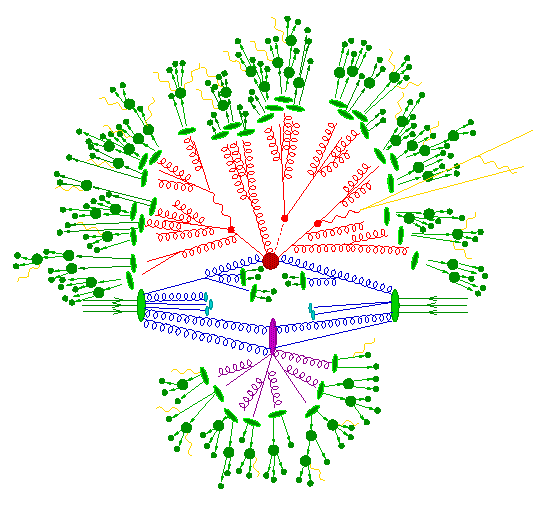
\includegraphics[width=0.90\textwidth]{Figures/LHC/HocheMCEG_final.pdf}
    \caption{This is a diagram of a simulated proton-proton collision. The hard collision is shown in the centre in red. In purple is the secondary hard scattering event. The parton shower is drawn in blue. Hadronisation is sketched in light green, and the subsequent hadron decays and final state particles are shown in dark green. Finally, the electromagnetic radiation is presented in yellow. This figure is from Reference~\cite{hoche2015introduction}.}
    \label{fig:MCEG}
\end{figure}

\subsubsection{Validation of V+jets production in Herwig7 with NLO multi-jet merging}
As part of the \ATLAS author qualification task, multi-leg merging at next-to leading order accuracy using the Matchbox framework in \herwig{7} was explored, with a focus on the vector boson plus jets process. Further details of the task and progression can be found on JIRA (\href{https://its.cern.ch/jira/browse/AGENE-1453}{\code{\textcolor{blue}{AGENE-1453}}}), and in the technical report of~\cite{Huang:2676143}.

\subsection{Monte Carlo samples}
\label{sec:montecarlopred}
This section provides a description of the event samples that are used for this analysis in the standard description of the ATLAS collaboration. These state-of-the-art predictions used to model the signal processes at detector-level and particle-level for this analysis, and to construct the response matrices that correct the data for detector effects. 
\subsection{\qqFourL}
The dominant \qqFourL process is simulated using the \SHERPA {2.2.2} event generator~\cite{Bothmann:2019yzt} with the \nnpdfnnlo{} set of PDFs~\cite{Ball:2014uwa}. The matrix elements are calculated at next-to-leading order accuracy for final states with zero and one jet, and at leading order accuracy for two- and three-jet final states. The different parton multiplicities are merged together and matched to the \SHERPA parton shower model based on the Catani-Seymour dipole factorization~\cite{Gleisberg:2008fv,Schumann:2007mg} using the MEPS@NLO prescription~\cite{Hoeche:2011fd,Hoeche:2012yf,Catani:2001cc,Hoeche:2009r}. A dedicated set of tuned parton-shower parameters developed by the \SHERPA authors are used. 
An alternate sample of the \qqFourL process is generated using  \POWHEGBOX v2~\cite{Alioli:2010xd,Melia:2011tj,Nason:2013ydw}. The sample is generated at NLO accuracy and interfaced to \PYTHIA 8.186 for the simulation of the parton shower, hadronization, and underlying event. The tuning parameters are set according to the AZNLO tune~\cite{STDM-2012-23}. The sample is corrected to higher order effects using a k-factor obtained with \textsc{Matrix} NNLO QCD prediction~\cite{Cascioli:2014yka,Grazzini:2015hta,Grazzini:2017mhc,Kallweit:2018nyv}. The $K$-factor is defined as the ratio of the NNLO cross-section to the NLO cross-section and applied as a function of \mFourL{}. 
Virtual electroweak NLO effects are accounted for by reweighting both samples with a mass-dependent $K$-factor. The high-order real electroweak contribution of $ZZ$ plus two jets is modelled separately in a \SHERPA{} {2.2.2} sample. 

\subsection{\ggFourL{}}
The gluon-gluon initiated \ggFourL{} process is modelled by \SHERPA{} 2.2.2 at leading order QCD for up to one additional parton emission. The \SHERPA parton shower model based on the Catani-Seymour dipole factorisation is used. Also included in this sample is the s-channel Higgs signal \ggS{} and its interference with the SM box diagram, which has a sizeable contribution above \unit{130}{\GeV}. For particle-level masses below \unit{130}{\GeV} the sample includes on the \ggFourL box diagram because the role of interference is negligible. An NLO QCD $K$-factor is derived using the ratio of the \SHERPA{} sample to an MCFM NLO sample~\cite{Campbell:2011bn}. This is applied as a mass-dependent weight.
An additional constant $K$-factor of 1.2 is applied to account for NNLO effects on the off-shell Higgs production cross-section~\cite{Passarino:2013bha,deFlorian:2016spz}. The sample has a generator cut of $\mll > 10~\GeV$ for same-flavour, opposite-charge lepton pairs. The contribution is below this cut is accounted for through the reweighting to MCFM prediction. Scale and PDF uncertainties are derived in the same way as for the \SHERPA{} \qqFourL{} sample.

\subsection{On-shell Higgs}
The resonant Higgs-boson production is an important process and is generated independently using the most precise description available. The SM Higgs can be produced via gluon-gluon fusion, vector-boson fusion (VBF), Higgstrahlung ($VH$), and in association with a top quark pair ($t\overline{t}H$). The \texttt{PDF4LHC15nnlo} and \texttt{PDF4LHC15nlo} PDF set~\cite{Butterworth:2015oua} are used, alongside AZNLO tune for all on-shell Higgs samples. The dominant gluon–gluon fusion production channel is simulated using the \powheg{} NNLOPS program~\cite{Hamilton:2013fea,Hamilton:2015nsa,Alioli:2010xd,Nason:2004rx,Frixione:2007vw} at NNLO accuracy in QCD, and matched to \pythia~\cite{Sjostrand:2014zea} for the simulation of the parton shower and non-perturbative effects. The sample is normalized to N$^3$LO in QCD cross-sections, which has been calculated for the gluon-fusion process, and corrected for NLO electroweak effects~\cite{deFlorian:2016spz,Anastasiou:2016cez,Anastasiou:2015ema,Dulat:2018rbf,Harlander:2009mq,Harlander:2009bw,Harlander:2009my,Pak:2009dg,Actis:2008ug,Actis:2008ts,Bonetti:2018ukf}. 
\powheg~\cite{Nason:2009ai,Alioli:2010xd,Nason:2004rx,Frixione:2007vw} is interfaced to \pythia{} for the vector-boson fusion process, the $WH$ and $ZH$ production process, and the small contribution from associated productions with a $t\overline{t}$ pair. All are estimated with matrix elements up to NLO in QCD. For VBF, the prediction is reweighted to an approximate-NNLO QCD cross-section with NLO electroweak corrections~\cite{Ciccolini:2007jr,Ciccolini:2007ec,Bolzoni:2010xr}. For VH, the prediction is normalized to an NNLO QCD cross-section calculation with electroweak NLO corrections~\cite{Ciccolini:2003jy,Brein:2003wg,Brein:2011vx,Denner:2014cla,Brein:2012ne}. 
The uncertainties for the on-shell Higgs samples are identical of that of a previous Higgs analysis, the largest of which are from the QCD scale and PDF uncertainties. A detailed description can be found in Reference~\cite{HIGG-2016-22}. 
%  The simulation achieves NNLO accuracy for arbitrary inclusive $gg\to H$ observables by reweighting the Higgs boson rapidity spectrum in \texttt{Hj-MiNLO}~\cite{Hamilton:2012np,Campbell:2012am,Hamilton:2012rf} to that of HNNLO~\cite{Catani:2007vq}.

\subsection{$VVV$ and $t\overline{t}V(V)$}
A smaller contribution to the four-lepton final state originates from triboson processes, and vector-boson production in association of top-quark pairs. These are referred to as $VVV$ (for $WWZ, WZZ$ and $ZZZ$) and $t\overline{t}V(V)$ (for $t\overline{t}Z$ and $t\overline{t}WW$) respectively. The tribon processes are modelled with \SHERPA{} 2.2.2 at NLO accuracy in QCD, with a Catani–Seymour dipole factorization based parton shower provided by \SHERPA{}. Two samples are provided for the  $t\overline{t}V(V)$ contribution. The first is simulated with \SHERPA{} 2.2.0 at LO accuracy up to final states with one additional jet. This sample is used to construct the response matrix used to correct the data for detector effects. The second prediction is produced with the \madgraph~2.3.3~\cite{Alwall:2014hca} generator at NLO accuracy interfaced to \PYTHIAV{8.210}~\cite{Sjostrand:2014zea}. This particle-level predictions of this sample is used to compared against the data for the interpretations of Section \ref{sec:interpretations}. A flat uncertainty of $\pm15\%$ to account for the differences between the two samples is is assigned.

\subsection{Corrections}
All MC events are processed through GEANT4~\cite{Geant4} to simulate the expected response of the ATLAS detector. Next, the samples are passed through the same object reconstruction and identification algorithms as the data and the analysis selection is applied. An illustration of the interface between MC simulation and data analysis is shown in Figure \ref{fig:dataMCflow}. Pile-up is simulated with \PYTHIAV{8.186} as inclusive inelastic $pp$ collisions. The events are then reweighted to reproduce the distribution of the mean number of interactions per brunch crossing (33.7 on average for the whole dataset). Lastly, events are  reweighted to account for the differences of the lepton reconstruction, identification, isolation, and vertex-matching efficiencies between data and simulation.

